% ==============================================================================
% CHAPTER 3: System Architecture & Unified Data Model
% ==============================================================================

\chapter{System Architecture}
\label{ch:system_arch}

\lettrine[lines=3]{A}{ key innovation} of the proposed automation platform is its decoupled architecture. Unlike traditional approaches that attempt to solve high-level strategic reasoning and sub-micron physical geometry placement in a single compiler pass, this framework divides the problem into separate strategic planning and physical execution layers. By abstracting the layout canvas into a symbolic grid, Large Language Models (LLMs) can perform spatial reasoning without calculating floating-point micron-level coordinates. The physical engine then resolves the symbolic grid into a DRC-clean physical design.

This chapter details the LayoutCopilot architecture, explaining the central data model that represents layouts symbolically, the four operational stages of the compiler, the dual interface modes (Qt GUI and MCP Server), the multi-agent system state transitions, and the deterministic physical backend compilation.

% ==============================================================================
\section[Decoupled Architecture Model]{The LayoutCopilot Decoupled Architecture Model}
\label{sec:arch_model}

Large Language Models excel at symbolic reasoning, semantic pattern matching, and strategic planning, but they perform poorly when executing precise arithmetic calculations in continuous space. In sub-micron analog layout, a coordinate rounding error of a single nanometer can cause catastrophic design rule violations (such as gate-to-contact spacing overlaps or active area enclosures), rendering the fabricated chip non-functional. 

To bridge this capability gap, our proposed LayoutCopilot framework decouples layout generation into two distinct domains (strategic symbolic planning and deterministic physical execution) executed across four compilation stages:
\begin{enumerate}
    \item \textbf{Stage 1: Input Ingestion (EDA Front-end):} Parses raw SPICE netlists, resolves PDK parameters, and performs isomorphic subgraph matching to detect symmetry structures.
    \item \textbf{Stage 2: LangGraph-Driven Multi-Agent Placer (AI Layer):} Strategic floorplanning and device row mapping using collaborative AI agents in a self-healing placer-critic loop.
    \item \textbf{Stage 3: Interactive Chatbot Co-Pilot (Designer Interface):} A PySide6 GUI that allows human designers to interactively refine layouts through natural language commands translated to XML actions.
    \item \textbf{Stage 4: Compaction \& Export Pipelines (Physical Layer):} A deterministic geometry engine that solves constraint graphs, sharing diffusions between adjacent fingers, and streams binary OASIS layouts or injects coordinates into Virtuoso via TCL.
\end{enumerate}

Let the set of devices to be placed be $\mathcal{M} = \{M_1, M_2, \dots, M_n\}$. In the symbolic planning phase, each device $M_i$ is mapped to a symbolic configuration:
\begin{equation}
    \mathcal{L}_{\text{sym}}(M_i) = \langle row_i, slot_i, orient_i \rangle
\end{equation}
where $row_i \in \{0, 1, \dots, N_{\text{rows}}-1\}$ represents the horizontal layout row, $slot_i \in \{0, 1, \dots, N_{\text{slots}}-1\}$ represents the relative position within that row, and $orient_i \in \{R0, MX, MY, R180\}$ represents the device orientation.

The physical layout engine maps this symbolic layout configuration to physical coordinates in continuous space:
\begin{equation}
    \mathcal{L}_{\text{phy}}(M_i) = \langle x_i, y_i, w_i, h_i \rangle \in \mathbb{R}^4
  \label{eq:physical_mapping}
\end{equation}
where $(x_i, y_i)$ is the lower-left origin of the device, and $w_i, h_i$ represent its calculated physical width and height (which depend on PDK variables and the number of gate fingers). 

This physical mapping is computed by solving a set of relative placement constraints:
\begin{equation}
    x_j - x_i \ge w_i + S_{ij} \quad \forall i, j \text{ where } slot_j > slot_i
\end{equation}
where $S_{ij}$ is the minimum design rule spacing required between the layers of device $M_i$ and $M_j$. 

Figure~\ref{fig:detailed_dataflow} illustrates the complete system dataflow and compilation stages, tracing the lifecycle of a design from SPICE schematic input down to physical GDSII/OASIS streaming.

\begin{figure}[H]
    \centering
    \fbox{\begin{tikzpicture}[
        node distance=1.2cm and 1.1cm,
        preproc/.style={draw=CodeBlue, fill=CodeBlue!8, text=CodeBlue!80!black, thick, rounded corners, minimum width=2.4cm, minimum height=1.1cm, align=center, font=\small\sffamily\bfseries, drop shadow={shadow xshift=1.5pt, shadow yshift=-1.5pt, fill=black!15}},
        agent/.style={draw=RoyalBlue, fill=LightBlueBg, text=AcademicBlue, thick, rounded corners, minimum width=2.4cm, minimum height=1.1cm, align=center, font=\small\sffamily\bfseries, drop shadow={shadow xshift=1.5pt, shadow yshift=-1.5pt, fill=black!15}},
        critic/.style={draw=WarmGold, fill=PaleGold!20, text=AcademicBlue, thick, rounded corners, minimum width=2.4cm, minimum height=1.1cm, align=center, font=\small\sffamily\bfseries, drop shadow={shadow xshift=1.5pt, shadow yshift=-1.5pt, fill=black!15}},
        solver/.style={draw=CodeGreen, fill=CodeGreen!10, text=CodeGreen!80!black, thick, rounded corners, minimum width=2.4cm, minimum height=1.1cm, align=center, font=\small\sffamily\bfseries, drop shadow={shadow xshift=1.5pt, shadow yshift=-1.5pt, fill=black!15}},
        ui/.style={draw=CopperAccent, fill=CopperAccent!8, text=CopperAccent!80!black, thick, rounded corners, minimum width=2.4cm, minimum height=1.1cm, align=center, font=\small\sffamily\bfseries, drop shadow={shadow xshift=1.5pt, shadow yshift=-1.5pt, fill=black!15}},
        arrow/.style={-Latex, line width=1.3pt, draw=AcademicBlue},
        feedbackarrow/.style={-Latex, line width=1.3pt, draw=WarmGold, dashed},
        looparrow/.style={-Latex, line width=1.3pt, draw=CodeGreen}
    ]
        % Background panel for AI planning space
        \fill[LightBlueBg!50, rounded corners=10pt, draw=RoyalBlue!20, dashed] (-1.6,-2.8) rectangle (5.9,0.8);
        \node at (2.2,0.5) [font=\tiny\sffamily\bfseries\color{RoyalBlue}] {Strategic AI Planner Space};

        % Nodes
        \node[preproc, align=center] (spice) {SPICE Netlist \\ Input};
        \node[agent, right=1.6cm of spice, align=center] (analyst) {Topology Analyst \\ (LangGraph)};
        \node[agent, below=1cm of analyst, align=center] (specialist) {Placement Specialist \\ (Symbolic Grid)};
        \node[critic, left=of specialist, align=center] (critic) {DRC Critic \\ (Self-Healing Loop)};
        
        \node[solver, right=1.6cm of specialist, align=center] (compactor) {Diffusion Compactor \\ (1D Solver)};
        \node[solver, below=1cm of compactor, align=center] (gdstk) {gdstk Exporter \\ (GDSII/OASIS)};
        \node[ui, left=of gdstk, align=center] (gui) {PySide6 Canvas \\ \& KLayout View};

        % Connect
        \draw[arrow] (spice) -- (analyst);
        \draw[arrow] (analyst) -- (specialist);
        \draw[arrow] (specialist) -- (critic);
        \draw[feedbackarrow] (critic) -- (specialist);
        \draw[arrow] (specialist) -- (compactor);
        \draw[arrow] (compactor) -- (gdstk);
        \draw[looparrow] (gdstk) -- (gui);
        \draw[looparrow] (gui) -- (specialist);
    \end{tikzpicture}}
    \caption{Detailed Dataflow and Control Loop of the Decoupled AI Layout Compiler.}
    \label{fig:detailed_dataflow}
\end{figure}
\newpage
\subsection{Stage 1: Input Ingestion \& PDK Parsing}

The compilation starts with the ingestion stage. The parser reads standard SPICE netlists and extracts net topologies, device characteristics (widths, lengths, finger counts), and PDK template options. It resolves these parameters into a unified database. A graph isomorphism algorithm detects symmetry structures like differential pairs and current mirrors, mapping them to hierarchical constraint sets. Figure~\ref{fig:parser_flowchart} details this parsing pipeline.

\begin{figure}[H]
    \centering
    \fbox{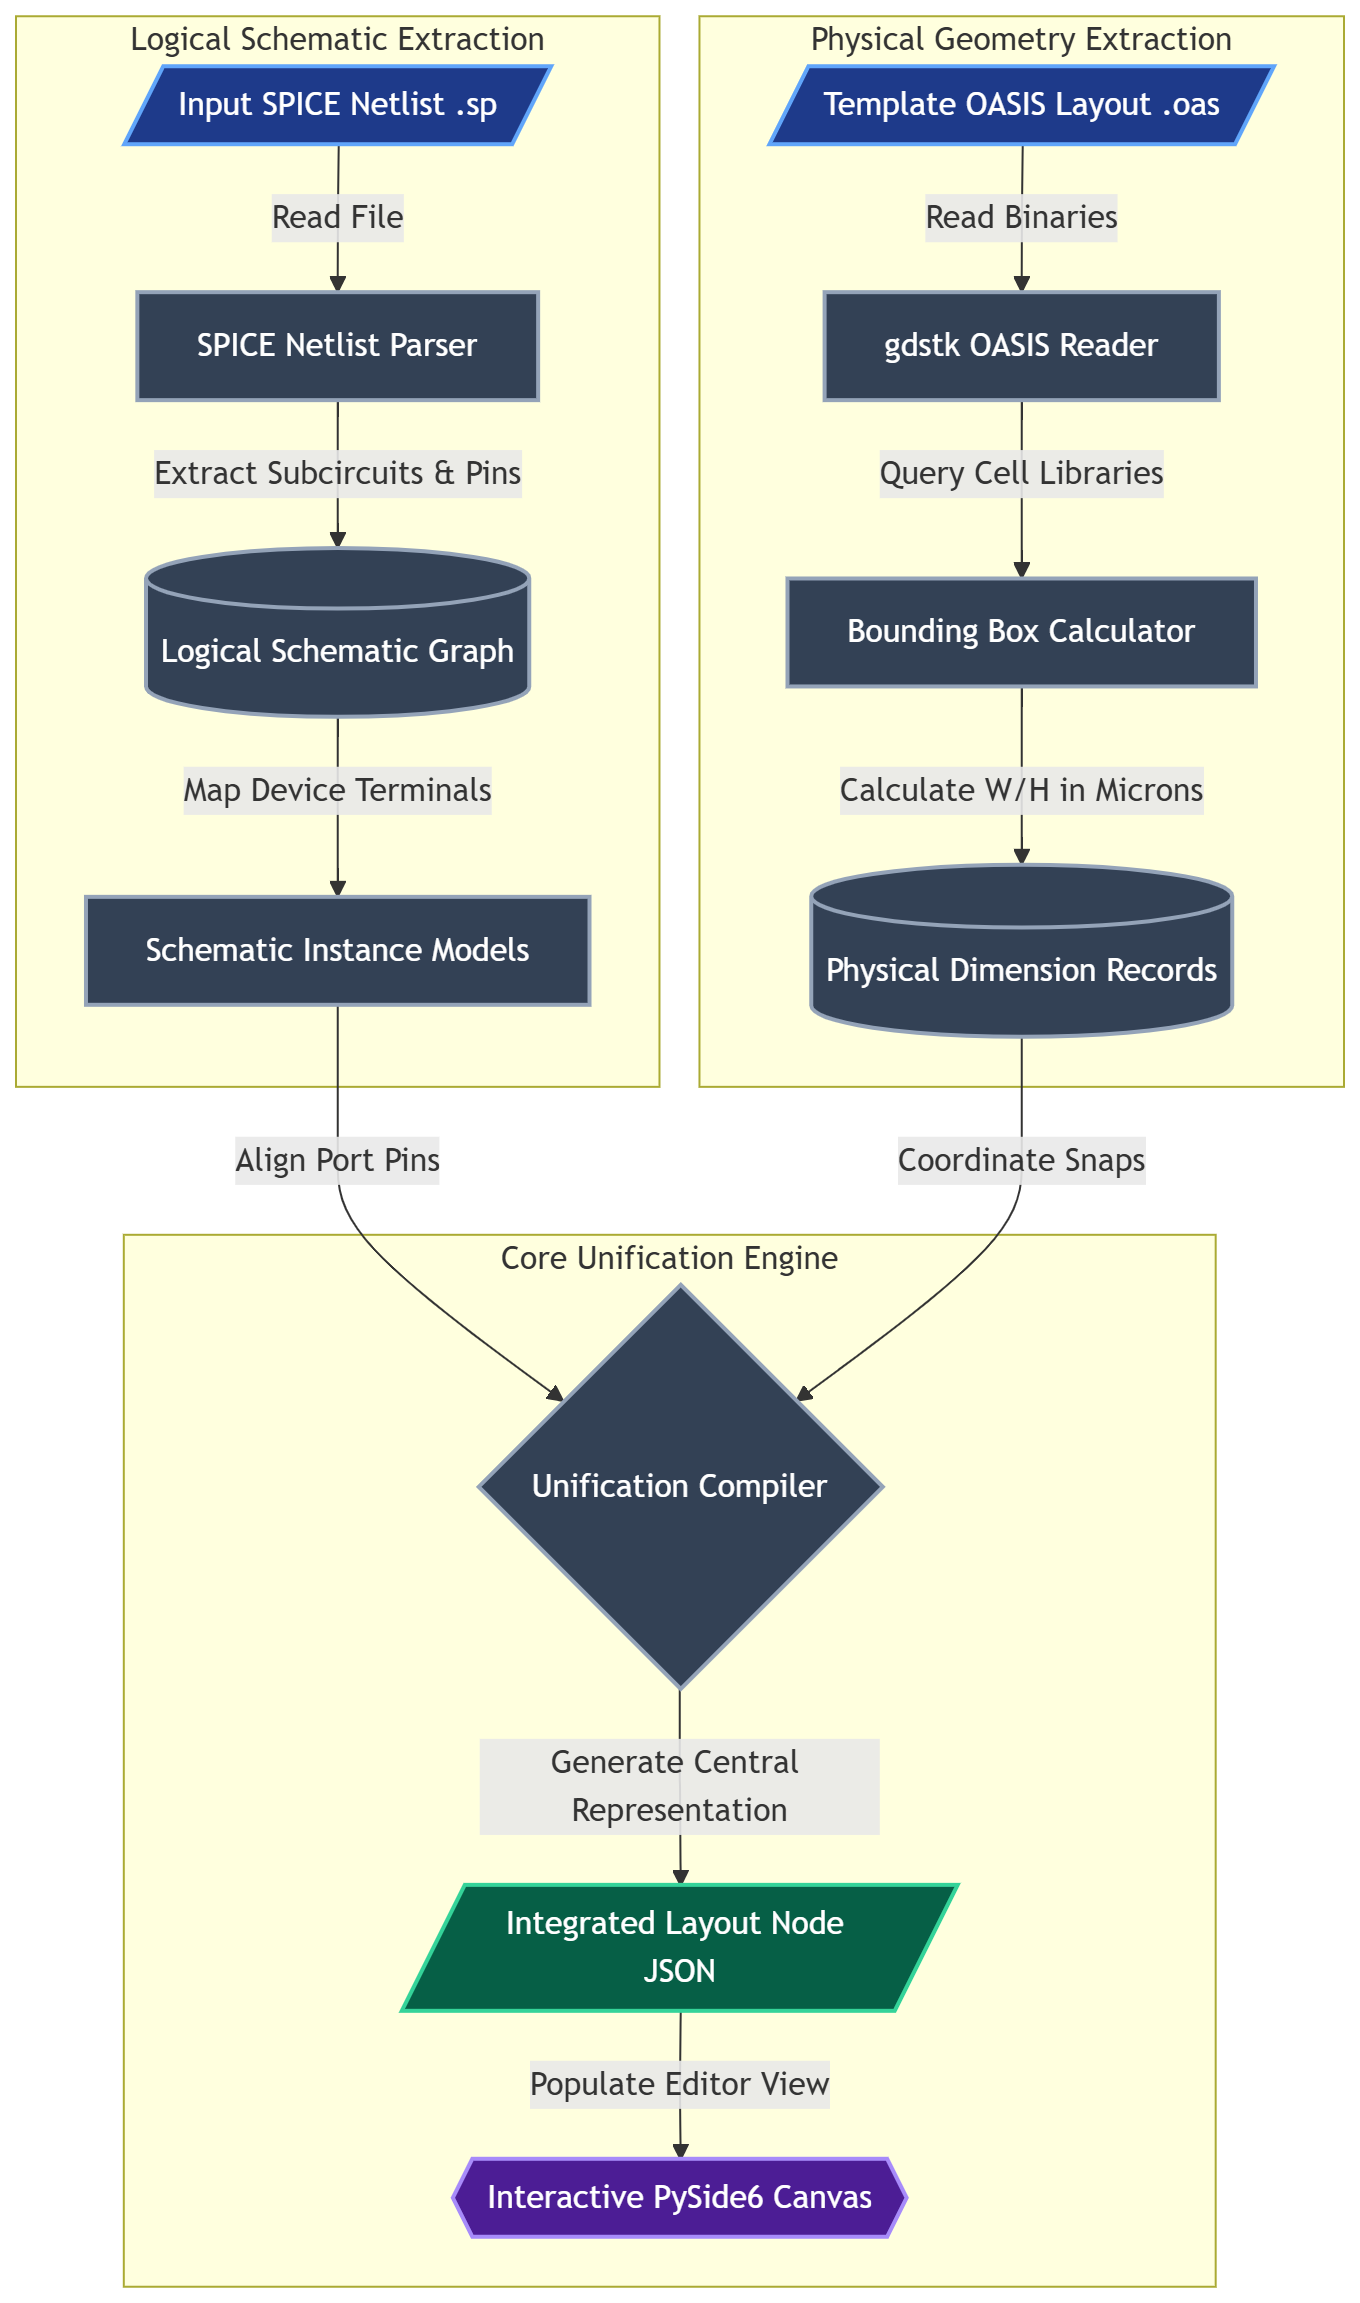
\includegraphics[width=13.5cm,height=16.5cm,keepaspectratio]{figures/parser.png}}
    \caption{Detailed flowchart of Stage 1 (Input Ingestion and Parser Flow) mapping schematics to PDK-compatible nodes.}
    \label{fig:parser_flowchart}
\end{figure}

% ==============================================================================
\section[Layer 2: AI Placement]{Layer 2: Strategic AI Placement Layer (LangGraph State Machine)}
\label{sec:ai_layer}

The strategic planning of the layout is governed by a multi-agent system implemented using LangGraph. LangGraph enforces a structured state-machine flow, which ensures that the agents collaborate in a predictable, self-healing loop. We define the graph state $S$ mathematically as a tuple of four elements:
\begin{equation}
    S = \langle P, C, F, H \rangle
\end{equation}
where $P$ is the set of current symbolic device placements, $C$ represents the active constraints, $F$ represents the history of critic feedback, and $H$ represents human overrides.

\subsection{Agent Prompt Design and Instructions}

Each agent within the LangGraph layer is driven by specific system prompts that define their role and scope:
\begin{itemize}
    \item \textbf{Topology Analyst Agent Prompt:} 
    \begin{quote}
        \textit{"You are an expert Analog IC Topology Analyst. Your task is to parse the input SPICE netlist and detect sub-block hierarchies. Identify differential pairs, current mirrors, and matched resistor/capacitor arrays. Output a structured constraint set containing symmetry pairings and matching groups. Do not define absolute physical coordinates."}
    \end{quote}
    \item \textbf{Placement Specialist Agent Prompt:}
    \begin{quote}
        \textit{"You are an Analog Layout Placement Specialist. You receive a list of devices, a set of constraints (symmetry, alignment, abutment), and a symbolic placement grid. Your task is to assign each device to a row index and slot index on the symbolic grid. Respect symmetry axes by placing paired devices symmetrically around the center slot. Output only the updated symbolic grid in JSON format."}
    \end{quote}
    \item \textbf{DRC Critic Agent Prompt:}
    \begin{quote}
        \textit{"You are a DRC Critic. Analyze the candidate symbolic placement. Check for adjacent spacing clearance, guard ring enclosures, and symmetry axis alignments. If a violation is detected, calculate the offset error and write an actionable feedback instruction (e.g., 'Move MM1 by +1 slot' or 'Insert dummy cell at slot 2'). if no violations exist, mark the state as DRC-clean."}
    \end{quote}
\end{itemize}
\newpage
The feedback loop routes execution between the Placement Specialist and the DRC Critic. The loop terminates when the DRC Critic returns a "DRC-clean" status, or when the iteration count exceeds a pre-set maximum ($T_{\text{max}} = 5$). When $T_{\text{max}}$ is exceeded, the system prompts the human designer in the chatbot panel to resolve the conflict.

Figure~\ref{fig:langgraph_transitions} illustrates the state transitions and agent routing rules of this multi-agent loop.

\begin{figure}[H]
    \centering
    \fbox{\begin{tikzpicture}[
        node distance=1.5cm and 2.0cm,
        startstate/.style={draw=CodeGreen, fill=CodeGreen!10, text=CodeGreen!60!black, thick, circle, minimum size=2.2cm, align=center, font=\small\sffamily\bfseries, drop shadow={shadow xshift=1.5pt, shadow yshift=-1.5pt, fill=black!15}},
        agentstate/.style={draw=RoyalBlue, fill=LightBlueBg, text=AcademicBlue, thick, circle, minimum size=2.2cm, align=center, font=\small\sffamily\bfseries, drop shadow={shadow xshift=1.5pt, shadow yshift=-1.5pt, fill=black!15}},
        endstate/.style={draw=CodeGreen!80!black, fill=CodeGreen!20, text=CodeGreen!60!black, thick, circle, minimum size=2.2cm, double, align=center, font=\small\sffamily\bfseries, drop shadow={shadow xshift=1.5pt, shadow yshift=-1.5pt, fill=black!15}},
        decision/.style={draw=WarmGold, fill=PaleGold!30, text=AcademicBlue, thick, diamond, aspect=2, minimum width=2.6cm, minimum height=1.3cm, align=center, font=\small\sffamily\bfseries, drop shadow={shadow xshift=1.5pt, shadow yshift=-1.5pt, fill=black!15}},
        arrow/.style={-Latex, line width=1.3pt, draw=AcademicBlue},
        feedbackarrow/.style={-Latex, line width=1.3pt, draw=WarmGold, dashed}
    ]
        % Nodes
        \node[startstate, align=center] (start) {Start / \\ Ingestion};
        \node[agentstate, right=of start, align=center] (analyst) {Topology \\ Analyst};
        \node[agentstate, right=of analyst, align=center] (specialist) {Placement \\ Specialist};
        \node[agentstate, below=of specialist, align=center] (critic) {DRC \\ Critic};
        \node[decision, left=of critic, align=center] (check) {DRC \\ Violations?};
        \node[endstate, left=of check, align=center] (done) {Execute \\ Compaction};

        % Connect
        \draw[arrow] (start) -- (analyst);
        \draw[arrow] (analyst) -- (specialist);
        \draw[arrow] (specialist) -- (critic);
        \draw[arrow] (critic) -- (check);
        
        \draw[feedbackarrow] (check) -- node[midway, above, font=\scriptsize\bfseries\color{WarmGold}] {Yes} (specialist);
        \draw[arrow] (check) -- node[midway, below, font=\scriptsize\bfseries\color{CodeGreen!60!black}] {No} (done);

    \end{tikzpicture}}
    \caption{LangGraph Agent State Transition and Feedback Loop.}
    \label{fig:langgraph_transitions}
\end{figure}
\newpage
\subsection{LangGraph Agent Collaborative Flow}

The multi-agent loop orchestrates the interaction between the Topology Analyst, Placement Specialist, and DRC Critic. The Placement Specialist proposes symbolic slot configurations, which are evaluated by the DRC Critic. Spacing and overlap violations are fed back as text prescriptions (e.g., "Shift MM1 by +1 slot") to guide the next iteration. Figure~\ref{fig:ai_placement_flowchart} shows the detailed decision and state flow within the placement agent.

\begin{figure}[H]
    \centering
    \fbox{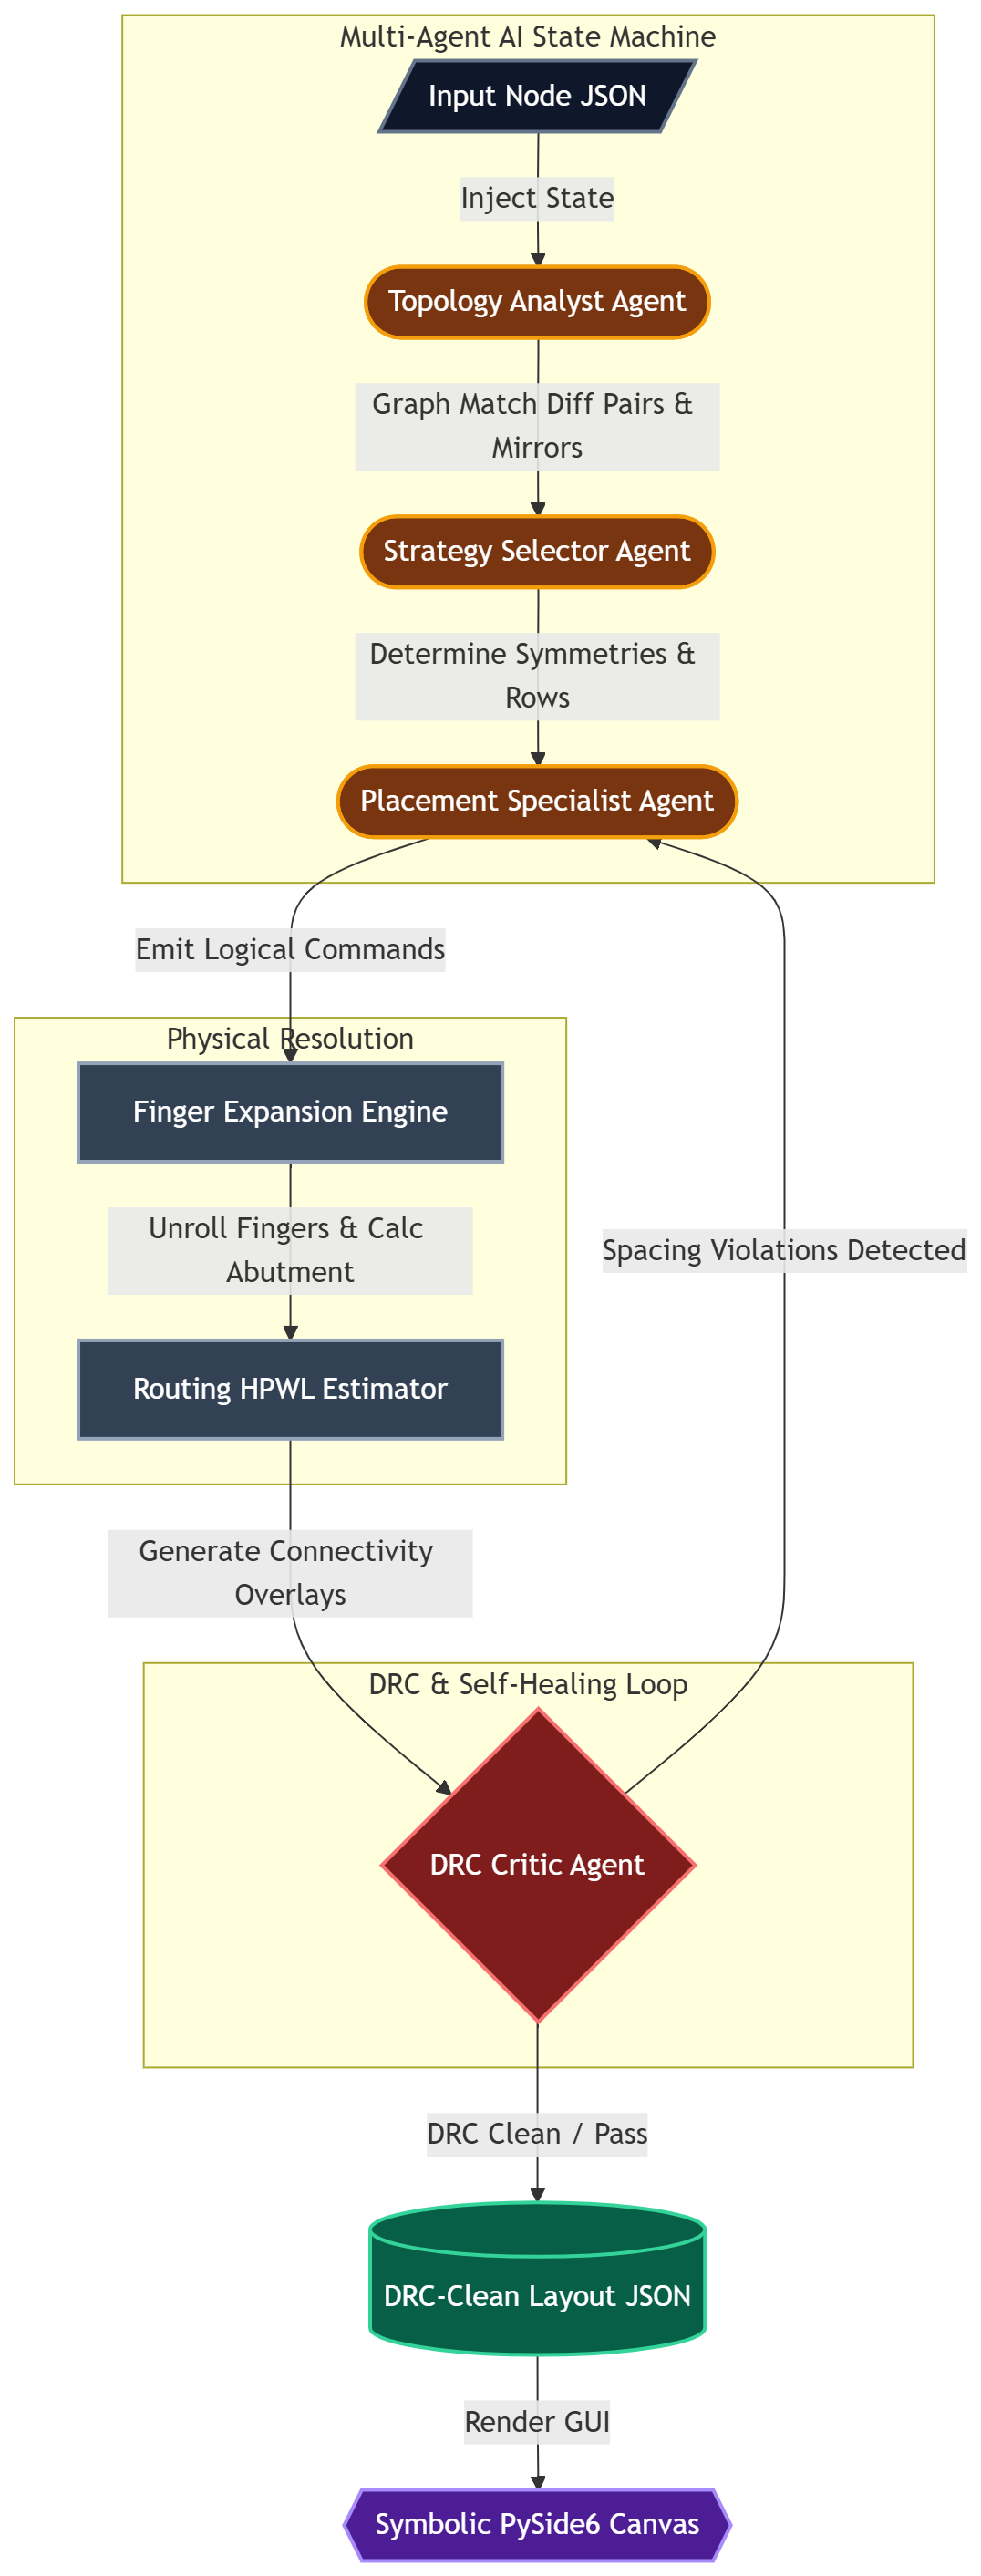
\includegraphics[width=13.5cm,height=16.5cm,keepaspectratio]{figures/AI_Placement.png}}
    \caption{Detailed flowchart of Stage 2 (LangGraph AI Placement) showing the self-healing Placer-Critic loop.}
    \label{fig:ai_placement_flowchart}
\end{figure}

% ==============================================================================
\newpage
\section[Layer 1: GUI]{Layer 1: User Interaction and Visualization GUI}
\label{sec:gui_layer}

The primary interface for the designer is a graphical editor built with PySide6 (Python bindings for Qt6). The interface consists of a dynamic schematic/layout viewer canvas, a design hierarchy tree, a parameter configuration panel, and an embedded chatbot panel for AI co-pilot interaction.

The PySide6 application implements the Model-View-Controller (MVC) design pattern:
\begin{itemize}
    \item \textbf{Model:} Exposes the central JSON-based intermediate data representation representing the layout state.
    \item \textbf{View:} Rendered using a `QGraphicsView` and `QGraphicsScene` canvas. Devices are represented as custom graphical rect items (`QGraphicsRectItem`) that designers can drag, drop, and rotate.
    \item \textbf{Controller:} Handles event callbacks and coordinates updates between the graphical view, local tools, and the background compilation workers.
\end{itemize}

To maintain a highly responsive user interface, the application uses an asynchronous threading model. Running LLM inference, parsing netlists, and invoking compilation pipelines can take from several hundred milliseconds to tens of seconds. If these tasks were executed on the main Qt GUI thread, the interface would freeze, leading to a poor user experience. 

We address this by separating the UI event loop from execution. The GUI thread handles only user gestures, coordinate drawing, and screen updates. All AI reasoning, physical compaction, and database operations are delegated to worker classes running on separate QThreads. Communication between the GUI thread and the QThreads is managed using Qt's thread-safe signal-and-slot mechanism, as shown in Figure~\ref{fig:threading_model}.

\begin{figure}[H]
    \centering
    \fbox{\begin{tikzpicture}[
        node distance=1.5cm and 1.5cm,
        gui/.style={draw=WarmGold, fill=PaleGold!25, text=AcademicBlue, thick, rounded corners, minimum width=3.2cm, minimum height=1.2cm, align=center, font=\small\sffamily\bfseries, drop shadow={shadow xshift=1.5pt, shadow yshift=-1.5pt, fill=black!15}},
        worker/.style={draw=RoyalBlue, fill=LightBlueBg, text=AcademicBlue, thick, rounded corners, minimum width=3.2cm, minimum height=1.2cm, align=center, font=\small\sffamily\bfseries, drop shadow={shadow xshift=1.5pt, shadow yshift=-1.5pt, fill=black!15}},
        cmdarrow/.style={-Latex, line width=1.3pt, draw=RoyalBlue},
        resarrow/.style={-Latex, line width=1.3pt, draw=CodeGreen}
    ]
        % Swimlanes/Panels
        \fill[PaleGold!10, rounded corners=8pt] (-2.0,-2.0) rectangle (2.0,2.0);
        \node at (0,1.7) [font=\tiny\sffamily\bfseries\color{WarmGold!80!black}] {Main GUI Thread};
        
        \fill[LightBlueBg!40, rounded corners=8pt] (3.0,-2.0) rectangle (7.0,2.0);
        \node at (5,1.7) [font=\tiny\sffamily\bfseries\color{RoyalBlue}] {Background QThread};

        % Nodes
        \node[gui, align=center] (gui) at (0,0) {Qt GUI Thread \\ (Event Loop / UI)};
        \node[worker, align=center] (worker) at (5,0) {QThread Worker \\ (AI Placer / Compactor)};
        
        \draw[cmdarrow] ($(gui.east)+(0,0.35)$) -- ($(worker.west)+(0,0.35)$) 
            node[midway, above, font=\scriptsize\bfseries\sffamily\color{RoyalBlue}] {1. Emit Command};
        \draw[resarrow] ($(worker.west)+(0,-0.35)$) -- ($(gui.east)+(0,-0.35)$) 
            node[midway, below, font=\scriptsize\bfseries\sffamily\color{CodeGreen!60!black}] {2. Return Result};
    \end{tikzpicture}}
    \caption{Asynchronous Threading Architecture using Qt Signals/Slots.}
    \label{fig:threading_model}
\end{figure}

The application also integrates with KLayout via a local TCP socket listener. When the compaction engine generates a new layout draft, it streams the geometry files (GDSII) and sends a reload command via the TCP socket. The running KLayout instance immediately refreshes its view, allowing the designer to inspect the physical GDSII layout side-by-side with the symbolic editor.
\newpage
\subsection{Stage 3: Interactive Chatbot Co-Pilot Loop}

The interactive review stage enables human-in-the-loop layout design. The user enters natural language instructions (e.g., "align MM1 and MM2 horizontally") into the PySide6 chatbot panel. The chatbot model translates these inputs into formal XML actions, which are queued and executed by the controller to update the canvas. The user can visually inspect the changes and trigger undo/redo actions dynamically. Figure~\ref{fig:chatbot_flowchart} shows the co-pilot loop.

\begin{figure}[H]
    \centering
    \fbox{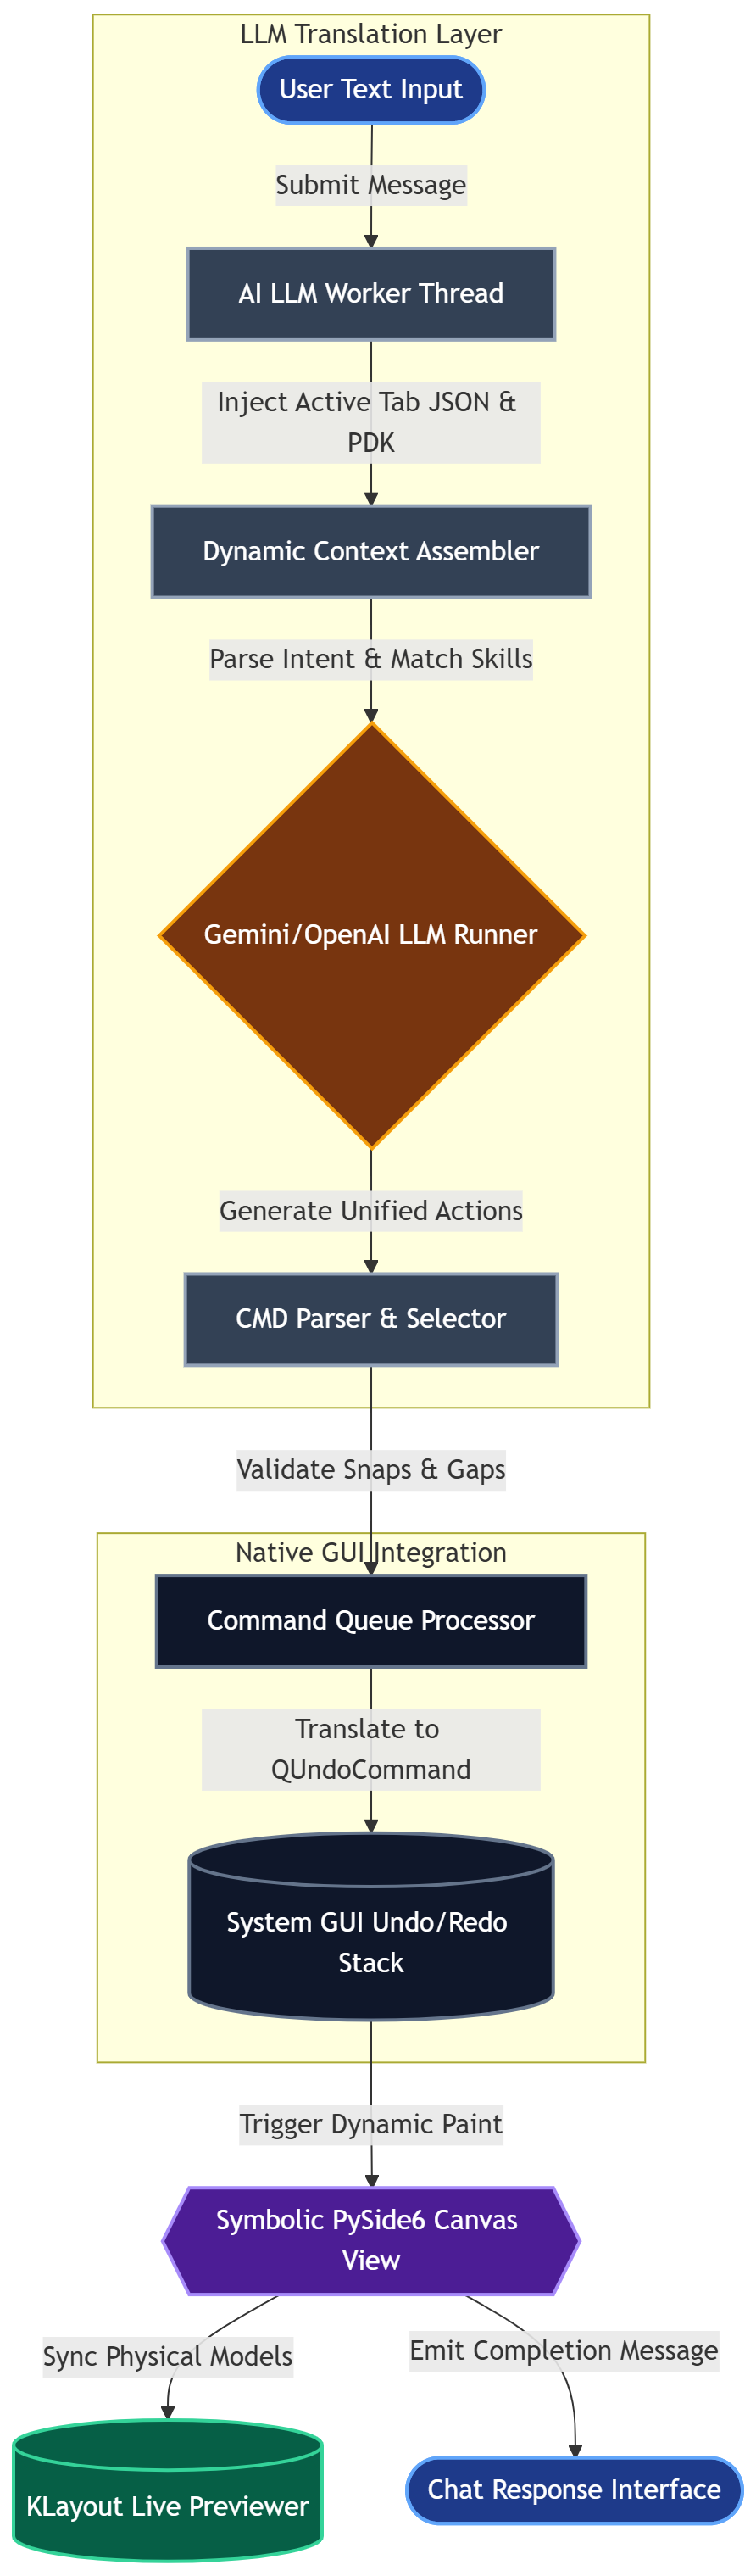
\includegraphics[width=13.5cm,height=16.5cm,keepaspectratio]{figures/ChatBot.png}}
    \caption{Flowchart of Stage 3 (Chatbot Co-Pilot) showing the interactive human-in-the-loop layout editing flow.}
    \label{fig:chatbot_flowchart}
\end{figure}

% ==============================================================================
\newpage
\section[Layer 3: Physical Compaction]{Layer 3: Deterministic Physical Compaction \& Extraction Engine}
\label{sec:physical_layer}

\subsection{Stage 4: Physical Compaction (Exporter)}

The final stage compiles the symbolic grid layouts into physical GDSII/OASIS files or injects coordinates directly into commercial databases. The physical compaction solver constructs directed constraint graphs, snapped to grid tracks, and applies diffusion-sharing rules to merge adjacent transistors. Figure~\ref{fig:tcl_oas_flowchart} details the Stage 4 physical backend.

\begin{figure}[H]
    \centering
    \fbox{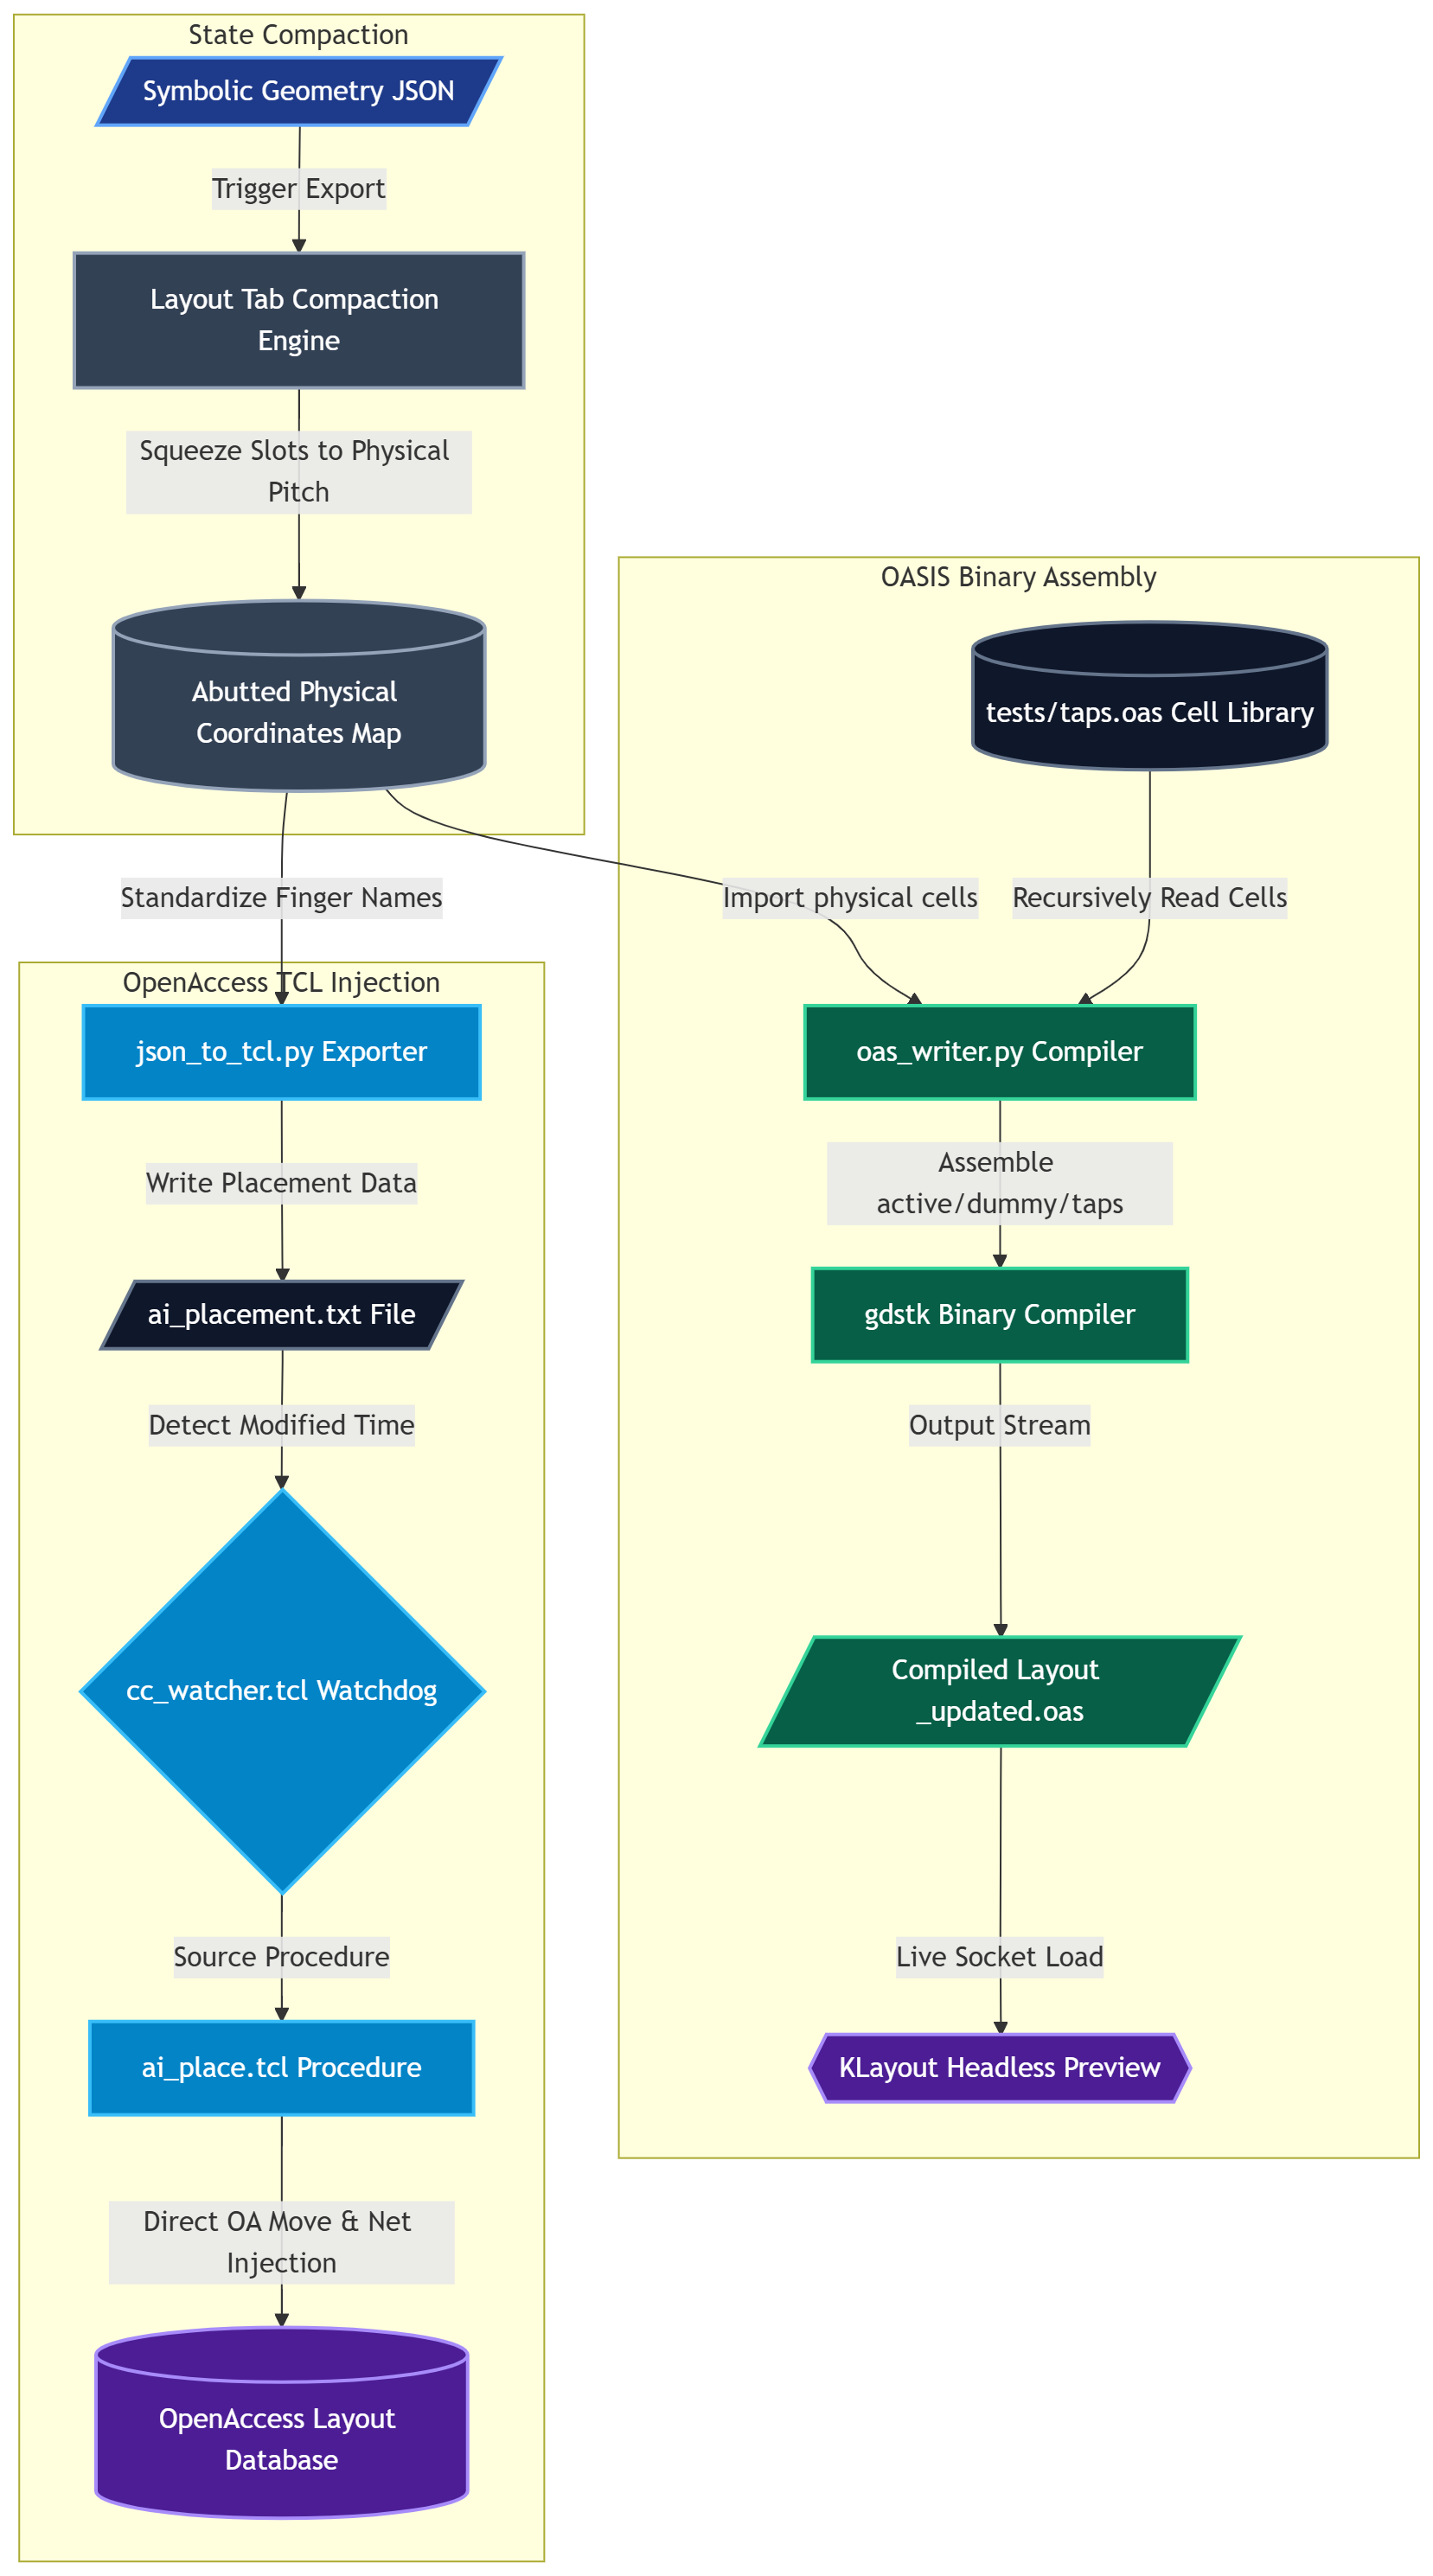
\includegraphics[width=13.5cm,height=15.5cm,keepaspectratio]{figures/tcl_oas.png}}
    \caption{Flowchart of Stage 4 (Compaction \& Export Pipelines) compiling symbolic slots into DRC-clean layout streams.}
    \label{fig:tcl_oas_flowchart}
\end{figure}

\subsection{1D Compaction using Constraint Graphs}

Layout compaction is formulated as a directed constraint graph $G_c = (V_c, E_c)$. Let the vertices $V_c$ correspond to the vertical boundaries of layout polygons, and the edges $E_c$ correspond to minimum spacing design rules. Let $x_i$ be the physical coordinate of boundary edge $i$. A spacing rule requiring a minimum distance $d_{ij}$ between edge $i$ and edge $j$ is modeled as $x_j - x_i \ge d_{ij}$.

The compilation steps for resolving the constraint graph are detailed in Algorithm~\ref{alg:compaction}.

\begin{thesisremark}{Algorithm 3.1: 1D Compaction Solver\label{alg:compaction}}
  Given a set of boundary edges $V_c$ and spacing constraints $E_c$:
  \begin{enumerate}
      \item Initialize coordinates: $x_i \gets 0$ for all $i \in V_c$.
      \item Sort vertices topologically since $G_c$ is a Directed Acyclic Graph (DAG).
      \item For each vertex $u$ in topological order:
      \item \quad For each outgoing edge $(u, v) \in E_c$ with weight $d_{uv}$:
      \item \quad\quad Update coordinate: $x_v \gets \max(x_v, x_u + d_{uv})$.
      \item Check for positive cycles (conflicting rules) using Bellman-Ford if sorting fails.
      \item Return coordinates $\mathbf{x}$.
  \end{enumerate}
\end{thesisremark}
\newpage
\subsection{Diffusion-Sharing Optimization}

To minimize layout area and reduce parasitic capacitance, the compaction engine includes a diffusion-sharing optimization stage. If two adjacent transistors $M_1$ and $M_2$ in the same row share an electrical net connection at their adjacent source/drain terminals, the engine merges their active areas (OD diffusion layers), removing the oxide isolation (STI) trench between them. The physical gate-to-gate spacing is reduced from the standard oxide-enclosure rule to the shared diffusion spacing rule. The merging logic is formalized in Algorithm~\ref{alg:diffusion_sharing}.

\begin{thesisremark}{Algorithm 3.2: Diffusion-Sharing Optimizer\label{alg:diffusion_sharing}}
  Given a row of placed devices $Row = [M_1, M_2, \dots, M_k]$:
  \begin{enumerate}
      \item Initialize $i \gets 1$.
      \item While $i < k$:
      \item \quad Get adjacent terminals: $T_r \gets Terminal_{\text{right}}(M_i)$, $T_l \gets Terminal_{\text{left}}(M_{i+1})$.
      \item \quad If $Net(T_r) == Net(T_l)$ and $M_i, M_{i+1}$ share the same active diffusion type (both NMOS or both PMOS):
      \item \quad\quad Mark boundary: $Merge(M_i, M_{i+1}) \gets \text{True}$.
      \item \quad\quad Update spacing constraint: $d_{i, i+1} \gets S_{\text{gap}}$.
      \item \quad Else:
      \item \quad\quad Mark boundary: $Merge(M_i, M_{i+1}) \gets \text{False}$.
      \item \quad\quad Update spacing constraint: $d_{i, i+1} \gets 2 \cdot L_{\text{enclosure}} + S_{\text{STI}}$.
      \item \quad Increment $i \gets i + 1$.
  \end{enumerate}
\end{thesisremark}

This merging reduces the junction area $A_d$ and perimeter $P_d$, which in turn minimizes the parasitic junction capacitance:
\begin{equation}
    C_{\text{db}} = A_d \cdot C_{\text{ja}} + P_d \cdot C_{\text{jp}}
\end{equation}
by up to $40\%$, improving circuit speed and matching performance.

% ==============================================================================
\newpage
\section[JSON Schema]{Central Intermediate Data Representation (JSON Schema)}
\label{sec:data_model}

The central source of truth shared between the frontend GUI, the LangGraph agents, and the physical exporters is the layout node JSON representation. This schema models transistors, dummies, and taps.

Listing~\ref{lst:json_schema} shows a sample transistor representation within this central data model, highlighting the separation between logical connectivity (\texttt{electrical}) and physical properties (\texttt{geometry}).

\begin{thesiscode}{Sample Transistor Entry in Layout JSON Schema\label{lst:json_schema}}{json}
{
  "id": "MM1",
  "type": "nmos",
  "is_dummy": false,
  "dummy_source": null,
  "electrical": {
    "gate": "NET_INP",
    "source": "NET_TAIL",
    "drain": "NET_OUTN",
    "bulk": "NET_VSS"
  },
  "geometry": {
    "x": 0.0,
    "y": 0.0,
    "width": 0.588,
    "height": 0.840,
    "orientation": "R0",
    "multiplier": 2,
    "nf": 2
  },
  "template_layout_index": 0,
  "layout_cell": "nfet_01v8"
}
\end{thesiscode}

\vspace{0.5cm}
\newpage
In addition to active devices, dummy transistors and substrate/well taps are modeled in the schema to ensure consistent physical boundary rules. Listing~\ref{lst:dummy_schema} shows a sample dummy device configuration.

\begin{thesiscode}{Sample Dummy Transistor Entry in JSON Schema\label{lst:dummy_schema}}{json}
{
  "id": "MDUMMY1",
  "type": "nmos",
  "is_dummy": true,
  "dummy_source": "NET_VSS",
  "electrical": {
    "gate": "NET_VSS",
    "source": "NET_VSS",
    "drain": "NET_VSS",
    "bulk": "NET_VSS"
  },
  "geometry": {
    "x": -1.2,
    "y": 0.0,
    "width": 0.588,
    "height": 0.840,
    "orientation": "R0",
    "multiplier": 1,
    "nf": 2
  },
  "template_layout_index": 0,
  "layout_cell": "nfet_01v8"
}
\end{thesiscode}

\vspace{0.5cm}
Key fields in this schema are:
\begin{itemize}
    \item \textbf{is\_dummy:} A boolean indicating if the device is active or a dummy padding transistor.
    \item \textbf{electrical:} Connects the terminals (Gate, Source, Drain, Bulk) to logical net names. This is used by the router and DRC checkers.
    \item \textbf{geometry.nf:} Number of gate fingers. This dictates how the unrolling engine expands the device.
\end{itemize}

% ==============================================================================
\newpage
\section[MCP Server Integration]{Model Context Protocol (MCP) Server Integration}
\label{sec:mcp_integration}

To support external LLM clients, the architecture integrates a Model Context Protocol (MCP) server. MCP is a stdio-based communication protocol that allows external models (e.g., Claude Desktop) to invoke local tools and access files securely. The MCP server exposes a tool registry, including tools such as \texttt{place\_device}, \texttt{align\_devices}, and \texttt{run\_drc}.

The communication uses JSON-RPC 2.0 packets over standard input/output. Listing~\ref{lst:mcp_rpc} shows an example of a tool execution exchange where the client invokes the \texttt{place\_device} tool.

\begin{thesiscode}{Sample MCP JSON-RPC Exchange\label{lst:mcp_rpc}}{json}
// Client Request
{
  "jsonrpc": "2.0",
  "method": "tools/call",
  "params": {
    "name": "place_device",
    "arguments": {
      "device_id": "MM1",
      "row": 0,
      "slot": 1
    }
  },
  "id": 1
}

// Server Response
{
  "jsonrpc": "2.0",
  "result": {
    "content": [
      {
        "type": "text",
        "text": "Successfully placed MM1 at row 0, slot 1. File layout_state.json updated."
      }
    ]
  },
  "id": 1
}
\end{thesiscode}

\vspace{0.5cm}
When a tool is executed, the server updates a shared state file (\texttt{layout\_state.json}). The PySide6 application monitors this file and immediately updates the graphical canvas. This synchronization enables a real-time, interactive co-pilot design loop.

% ==============================================================================
\section[Security Boundaries]{Security Boundaries and Sandbox Isolation in MCP}
\label{sec:mcp_security}

\begin{thesiscallout}{Security Boundaries and Sandbox Isolation}
Integrating Large Language Models with local CAD tools poses security risks. Because LLMs can generate arbitrary code and execute tool calls, exposing direct system access (e.g., bash terminals or system commands) to the model could lead to malicious or unintended actions, such as overwriting critical PDK source files or deleting design databases.

To mitigate these risks, the proposed architecture implements strict security boundaries:
\begin{enumerate}
    \item \textbf{Stdio Isolation:} The MCP server communicates with the LLM client exclusively through standard input/output (stdio). There is no direct network socket or remote execution channel between the external client and the local system, limiting the attack surface.
    \item \textbf{Schema-based Tool Validation:} The LLM cannot execute arbitrary scripts on the host system. It is restricted to the specific API schema defined in the tool registry (e.g., placing cells or running DRC checks). The MCP server acts as a gatekeeper, parsing and validating the JSON parameters before translating them into physical commands:
    \begin{equation}
        \mathbf{x}_{\text{args}} \in \text{Registry\_Schema} \implies \text{Execute Tool}(\mathbf{x}_{\text{args}})
    \end{equation}
    If the parameters do not match the expected schema types, the command is immediately rejected with a JSON-RPC error.
    \item \textbf{File-system Sandboxing:} The MCP server is confined to the active project workspace directory. It cannot read or write files outside this sandbox, protecting the user's home directories and PDK system files.
\end{enumerate}
This sandboxed integration ensures that the AI co-pilot operates safely, protecting designer databases and PDK installations.
\end{thesiscallout}

